%% For double-blind review submission, w/o CCS and ACM Reference (max submission space)
\documentclass[sigplan,review]{acmart}\settopmatter{printfolios=true,printccs=false,printacmref=false}
%% For double-blind review submission, w/ CCS and ACM Reference
%\documentclass[sigplan,review,anonymous]{acmart}\settopmatter{printfolios=true}
%% For single-blind review submission, w/o CCS and ACM Reference (max submission space)
%\documentclass[sigplan,review]{acmart}\settopmatter{printfolios=true,printccs=false,printacmref=false}
%% For single-blind review submission, w/ CCS and ACM Reference
%\documentclass[sigplan,review]{acmart}\settopmatter{printfolios=true}
%% For final camera-ready submission, w/ required CCS and ACM Reference
%\documentclass[sigplan]{acmart}\settopmatter{}


%% Conference information
%% Supplied to authors by publisher for camera-ready submission;
%% use defaults for review submission.
\acmConference[LFM-NL'18]{Lorentz Formal Methods in the Netherlands }{September 03-04, 2018}{Leiden, NL}
\acmYear{2018}
\acmISBN{} % \acmISBN{978-x-xxxx-xxxx-x/YY/MM}
\acmDOI{} % \acmDOI{10.1145/nnnnnnn.nnnnnnn}
\startPage{1}

%% Copyright information
%% Supplied to authors (based on authors' rights management selection;
%% see authors.acm.org) by publisher for camera-ready submission;
%% use 'none' for review submission.
\setcopyright{none}
%\setcopyright{acmcopyright}
%\setcopyright{acmlicensed}
%\setcopyright{rightsretained}
%\copyrightyear{2018}           %% If different from \acmYear

%% Bibliography style
\bibliographystyle{ACM-Reference-Format}
%% Citation style
%\citestyle{acmauthoryear}  %% For author/year citations
%\citestyle{acmnumeric}     %% For numeric citations
%\setcitestyle{nosort}      %% With 'acmnumeric', to disable automatic
                            %% sorting of references within a single citation;
                            %% e.g., \cite{Smith99,Carpenter05,Baker12}
                            %% rendered as [14,5,2] rather than [2,5,14].
%\setcitesyle{nocompress}   %% With 'acmnumeric', to disable automatic
                            %% compression of sequential references within a
                            %% single citation;
                            %% e.g., \cite{Baker12,Baker14,Baker16}
                            %% rendered as [2,3,4] rather than [2-4].


%%%%%%%%%%%%%%%%%%%%%%%%%%%%%%%%%%%%%%%%%%%%%%%%%%%%%%%%%%%%%%%%%%%%%%
%% Note: Authors migrating a paper from traditional SIGPLAN
%% proceedings format to PACMPL format must update the
%% '\documentclass' and topmatter commands above; see
%% 'acmart-pacmpl-template.tex'.
%%%%%%%%%%%%%%%%%%%%%%%%%%%%%%%%%%%%%%%%%%%%%%%%%%%%%%%%%%%%%%%%%%%%%%


%% Some recommended packages.
\usepackage{booktabs}   %% For formal tables:
                        %% http://ctan.org/pkg/booktabs
\usepackage{subcaption} %% For complex figures with subfigures/subcaptions
                        %% http://ctan.org/pkg/subcaption


\begin{document}

%% Title information
\title[Short Title]{Saving the World}         %% [Short Title] is optional;
                                        %% when present, will be used in
                                        %% header instead of Full Title.
%\titlenote{with title note}             %% \titlenote is optional;
                                        %% can be repeated if necessary;
                                        %% contents suppressed with 'anonymous'
\subtitle{A long and windy road towards sustainability and formal verification in practice}                     %% \subtitle is optional
%\subtitlenote{with subtitle note}       %% \subtitlenote is optional;
                                        %% can be repeated if necessary;
                                        %% contents suppressed with 'anonymous'


%% Author information
%% Contents and number of authors suppressed with 'anonymous'.
%% Each author should be introduced by \author, followed by
%% \authornote (optional), \orcid (optional), \affiliation, and
%% \email.
%% An author may have multiple affiliations and/or emails; repeat the
%% appropriate command.
%% Many elements are not rendered, but should be provided for metadata
%% extraction tools.


%% Author with two affiliations and emails.
\author{Marko van Eekelen}
%\authornote{}          %% \authornote is optional;
                                        %% can be repeated if necessary
%\orcid{nnnn-nnnn-nnnn-nnnn}             %% \orcid is optional
\affiliation{
  \position{Full Professor, Head of Department}
  \department{Computer Science Department}             %% \department is recommended
  \institution{Faculty of Management, Science and Technology; Open University of The Netherlands}           %% \institution is required
  \streetaddress{}
  \city{Heerlen}
  \state{}
  \postcode{}
  \country{}                   %% \country is recommended
}
\email{Marko.vanEekelen@ou.nl}         %% \email is recommended


\affiliation{
  \position{Associate Professor}
  \department{Digital Security}             %% \department is recommended
  \institution{Institute for Computing and Information Sciences, Radboud University}           %% \institution is required
%  \streetaddress{}
  \city{Nijmegen}
  \state{}
  \postcode{}
  \country{}                   %% \country is recommended
}
\email{marko@cs.ru.nl}         %% \email is recommended


%% Abstract
%% Note: \begin{abstract}...\end{abstract} environment must come
%% before \maketitle command
\begin{abstract}
My research is spread over two universities, mainly in the following two different research areas: 
\begin{itemize}
\item \emph{Resource consumption analysis} 
\item \emph{Formal verification methods for verifying security and correctness in cyber physical systems}. 
\end{itemize}
\end{abstract}


%% 2012 ACM Computing Classification System (CSS) concepts
%% Generate at 'http://dl.acm.org/ccs/ccs.cfm'.
\begin{CCSXML}
<ccs2012>
<concept>
<concept_id>10011007.10011006.10011008</concept_id>
<concept_desc>Software and its engineering~General programming languages</concept_desc>
<concept_significance>500</concept_significance>
</concept>
<concept>
<concept_id>10003456.10003457.10003521.10003525</concept_id>
<concept_desc>Social and professional topics~History of programming languages</concept_desc>
<concept_significance>300</concept_significance>
</concept>
</ccs2012>
\end{CCSXML}

\ccsdesc[500]{Software and its engineering~General programming languages}
\ccsdesc[300]{Social and professional topics~History of programming languages}
%% End of generated code


%% Keywords
%% comma separated list
\keywords{formal, practical, sustainable}  %% \keywords are mandatory in final camera-ready submission


%% \maketitle
%% Note: \maketitle command must come after title commands, author
%% commands, abstract environment, Computing Classification System
%% environment and commands, and keywords command.
\maketitle


\section{Introduction}

\subsection{Computer Science Research at the Open University }
The OU CS department has an emerging research group within the Netherlands. Only since 2009 de OU formally has a disciplinary research task. Since 2014 the author is chairing the OU Computer Science Department with the intention that research at the Open University is just as important as education. This has lead to a growth of the department to a current size of over 30 members (4 full professors, 1 associate professor, 17 assistant professors, 5 lecturers,  4 postdocs, 13 external Ph.D. students) performing research in 3 focal points:

\begin{itemize} 
\item Learning (in 3 topics: Tools for Supporting Learning, Computer Science Education, Computer Science Didactics),  
\item Resilience - Trustworthy Systems (in 2 topics: Verification, Security \& Privacy) 
\item  Innovation (Artificial Intelligence, Machine Learning). 
\end{itemize}

The research is embedded in the Faculty of Management, Science and Technology promoting a culture of interdisciplinary research.

The members of the department recently acquired several grants (on Regional, National, European and American level) among which a Rubicon and a Veni grant.


\section{Resource Consumption Analysis}
Functional properties of programs are widely studied. It is however less common to study non-functional properties of code. Recently, the resources studied are diversifying \citep{Dagstuhl2017}. In particular, the study of the consumption of other resources than time is an opening field. Studying resources such as memory and energy seems to the most promising \citep{MarkoDagstuhl2017-Energy}.

 From the practical point of view, the results discussed in \citep{Shkaravska201415} improve polynomial resource analysis of computer programs as presented in \cite{shkarav-LMCS}. There the authors consider the size of output as a polynomial function on the sizes of inputs \citep{DBLP:datatype, DBLP:sizes}. In the NL NWO AHA project (2006-2011), the EU Charter Artemis project (2009-2012) and the NL GoGreen IOP GenCom project (2011-2015) the ResAna tool \citep{DBLP:tlca,DBLP:testing,DBLP:testinference,DBLP:Resana} was developed that applies polynomial interpolation to generate an upper bound on Java loop iterations. The tool requires the user to input the degree of the solution. In \citep{Shkaravska201415}  a partial result for that was provided. The results of recent work \citep{Shkaravska2018} make it possible to automatically obtain the degree of the polynomial in all cases for quadratic algebraic difference equation with constant coefficients.
 
Building upon this work, the focus moved from size, memory and loop bounds to sustainability of software \citep{bernardvangastel} in general and of energy consumption analysis  in particular.

\subsection{A Moral Appeal}
Computer Science is not the  most sustainable discipline, to say the least. Every few years new equipment 'has' to be bought. The energy consumption due to digital equipment is seldom an issue. In software development energy consumption is rarely an issue. Instead of paying attention to the sustainability of software in such a way that an important design concern is that during the software life cycle as less as possible energy is consumed, the sole focus seems to be to keep legacy systems running in terms of functionality whatever the influence is on energy consumption. 

As a discipline we need to do better with respect to sustainability. In fact, I would like to make a moral appeal for performing research in the area of energy analysis consumption paraphrasing famous words of John F. Kennedy: 

\indent
{"\emph{And so my fellow Formal Method researchers: ask not what the world can do to reduce the
energy consumption for you - ask how you can apply Formal Methods to reduce the energy consumption of
the world: ask not what other researchers will do for you, but what together we can do for reducing
the energy consumption of man.}"
}

The good news is that interest in energy consumption and in greenIT in the Netherlands is growing, e.g. at the Free University of Amsterdam \citep{DBLP:conf/greens/MoghaddamLB18}, at the Software Improvement Group \citep{DBLP:conf/ict4s/KalaitzoglouBV14}, at Utrecht University \citep{DBLP:conf/sac/JagroepWJFV15, DBLP:conf/icse/JagroepBWLBBV17} and at the Open University.

\subsection{Energy Consumption Analysis at the Open University}

Building upon practical resource analysis work \citep{DBLP:conf/jtres/KerstenSGME12} a research track on static analysis of energy consumption. This started with defining a suited Hoare logic that enabled a safely approximating static analysis \citep{fopara14-kersten-copy}. This resulted in a webtool, ECAlogic \citep{foal14-schoolderman}, that made it possible to derive energy consumption bounds for small systems (hardware components controlled by a software application) in a  hardware-parametric way. Due to this work the focus of the research changed to analysing IT controlled systems parametrised by hardware finite state machine models \citep{fopara16-vangastel}. The corresponding approach was to focus on systems with multiple components, model the components and 
analyse the control software to estimate the energy consumption of the system. Using dependent types the analysis was made ready for a practical, precise and parametric energy analysis of IT controlled systems \citep{bvg16}. In working towards actual practice a first, small case study revealed that instead of doing a full analysis it can be worthwhile to focus solely on finding energy hot spots and energy bugs \citep{Gastel:2018:DEB:3191697.3213805}. 

The OU memory and energy consumption analysis work was disseminated at the 2013 IPA Winterschool on Software Technology in Eindhoven, at the  2016 EU COST action TACLe Summerschool  in Vienna and at the 2017 IPA Fall Days on System and Software Analysis.



\subsection{Formal verification methods for verifying security and correctness in cyber physical systems at Radboud Unversity}

My Radboud research in formal verification started with work on a dedicated proof assistant for the functional programming language Clean with special support for generic type classes and explicit strictness \citep{DBLP:conf/agtive/MolE99, DBLP:conf/sfp/KesterenEM04, DBLP:conf/ifl/EekelenM05}. In the context of LaQuSO (Laboratory for Quality Software) we were able to verify the core decision algorithm of the Dutch Storm Surge Barrier 'Maeslantkering' protecting the Rotterdam area against flooding. The algorithm was formally specified in Z. We checked the code against the specification and we validated the specification. As a result firstly some minor changes were needed both in the specification and in the code and secondly a scenario popped up from model checking in which the barrier would  not close according to the specification while it should close according to the experts \citep{DBLP:conf/icfem/MadlenerSE10}. Everything was fixed such that the Dutch are saved from 'getting their feet wet'.

Currently, together with Herman Geuvers I am leading the STW Sovereign project (2016-2020) supported by RWS (the Dutch ministry of Transport, Public Works and Water Management) and NRG (the Dutch Nuclear Research Group). 
The
goal of this project is to develop verification techniques for safety critical software based on the following challenging principles.
Verification should be (1) scalable (costs
should not grow exceedingly as the size of the system
increases), (2) compositional (global properties
are directly inferable from local properties of
the subsystems), (3) incremental (the verification
process can be performed iteratively while previous
intermediate results are still usable), and (4)
effective (the proposed methodology will be applied
successfully in some real-world case studies).
The fundamental idea of our proposal can be
illustrated best with our motto: �Scalability through
modularity�. Modularity is commonly recognized
as the key for managing complex software systems.
With regards to programs, we will elaborate on the concept of design pattern (a description of
a solution to a recurring problem) as a modularizing
construct. We will investigate both general
and security specific design patterns, and develop
accompanying proof patterns that simplify the formal
verification process.
Moreover, as an follow-up of our work on the
formalization of the C11 standard, we aim to  make an important step in improving the scalability of the C verification process.

\begin{figure}
\begin{center}
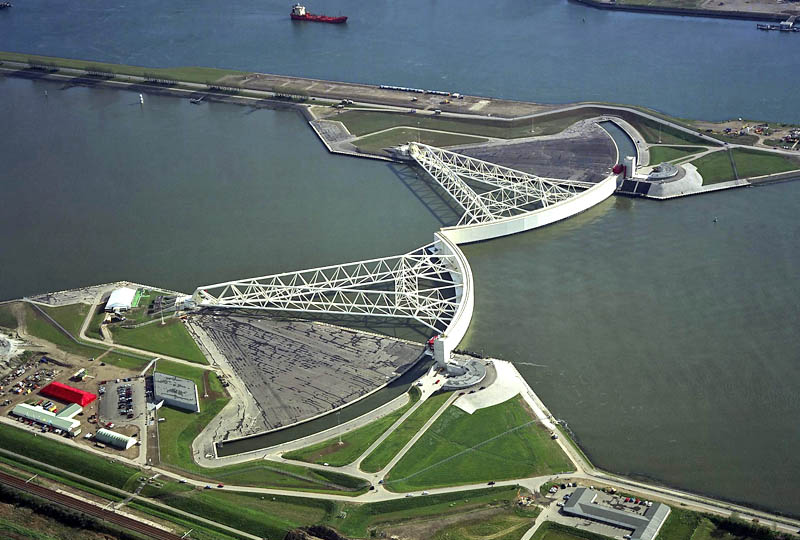
\includegraphics[scale=.27]{Maeslantkering}
\caption{Maeslantkering.}\label{fig:kering}
\end{center}
\end{figure}

\section{Moral Discussion}
Answer the following questions:
\begin{itemize}
\item Is n't it about time that IT starts saving the world instead of consuming it? 
\item Is n't it about time that IT starts saving the world before it is too late?
\item Is n't it about time that designs and implementations of safety critical cyber physical systems are subject to formal verification on a regular basis?
\end{itemize}

With every 'yes' we contribute to saving the world{\ldots}.
%% Bibliography
\bibliography{bibfile,common}
\bibliographystyle{plain}

%%% Appendix
%\appendix
%\section{Appendix}

%Text of appendix \ldots

\end{document}
